\documentclass[titlepage]{article}
\usepackage[left=15mm,right=15mm,top=1in,bottom=1in, margin=1in]{geometry}
\usepackage{graphicx}
\usepackage{pbox}
\usepackage{amssymb}
\usepackage{amstext}
\usepackage{amsthm}
\usepackage{amsmath}
\usepackage{enumerate}
\usepackage{fancyhdr}
\usepackage{extarrows}
\usepackage{setspace}

\title{Stone Identification App \\
	High-Level Architectural Design}
\author{Genevieve Okon (okong), Sydney Lieng(liengsn),\\
	Niko Savas(savasn), Nick Lago(lagond),\\
	Eric Le Fort(leforte)}
\date{\today}

\begin{document}
\maketitle
\newpage
\tableofcontents
\newpage


\section{Introduction}~\\
This document will explain the design of the Stone Identification App using, Use Case Diagram, Analysis Class Diagram, Architectural Design and Class Responsibility Collaboration Cards. 

\subsection{Purpose}
The purpose of this document is to describe the design architecture of the Stone Identification App. This will be achieved through a series of different diagrams and analysis techniques. The indented audience for this document is the software implementation team as well as the client.

\subsection{System Description}
The system that will be discussed in this report is that of the Stone Identification App. The system will be composed of multiple expert classes. Each of these classes will have access to a database containing a list of rocks and the details pertaining to those rocks. When a customer inputs information about a rock the system will use these experts to give a list of possible rocks they may have found. The user will be able to keep information on rocks they have found on a separate database held on local storage devices. The system will be designed as an android application. It will be able to be used on any android devices and will be purchased through the android app store. 

\subsection{Overview}
This document has 4 sections not including this one. Each section either contains design diagrams or an explanation that will further describe the architecture of the Stone Identification App. Each section will provide insight into a key aspect of design with the goal of preparing the software team to implement the design.
\begin{itemize}
	\item \textbf{Use Case:} This document will show who interacts with the system as well as the intended results of those interactions through Use Case Diagrams
	\item \textbf{Analysis Class Diagram:} The Analysis Class Diagram will outline which classes will be a boundary, controller or entity class and show their connections to one another
	\item \textbf{Architectural Design Class:} This section will show the overview of the overall design, and justification for the choice of this design
	\item \textbf{Class Responsibility Collaboration Cards} The use of these cards will show what the classes that make up the Stone Identification App key responsibilities are and what other classes they interact with
\end{itemize}


\newpage
\section{Use Case Diagram}~\\

  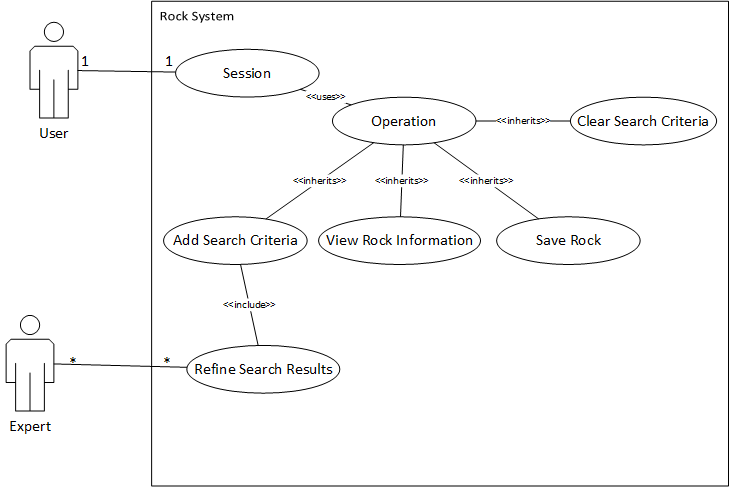
\includegraphics[scale = 0.5]{../resources/UseCaseDiagram.png}
  \subsection{Session}
    When the user opens the app, a session is started. During the session, the user can manage their search criteria to identify a rock, with information such as colour, size, and texture. The session is terminated when the user closes the app or is finished with their search.
  \subsection{Operation}
    The operation is an abstract use case. It is extended by clear search criteria, add search criteria, view rock information,view collection, and save rock.
  \subsection{Add Search Criteria}
    The user can add information about the rock to the search criteria to refine the list of possible matches. The list of possible matches is generated by both internal and external experts ("internal experts" are built in to the application, while "external experts" are actors upon the application providing context and data).
  \subsection{Refine Search Results}
    This use case is implemented by all external experts contributing to the application. Given a set of inputs, an expert can refine a set of search results to only include those that match the inputs.
  \subsection{View Rock Information}
    The user can view detailed information about any given rock included in the list of matches or their collection. The information displayed is sourced from the data store of the application.
  \subsection{View Collection}
    The user can view their collection of saved rocks. This provides a shortlist of rocks that have been added using the "Save Rock" operation. 
  \subsection{Save Rock}
    The user can, at any time, add a rock to their collection.


\section{Analysis Class Diagram}~\\
 \includegraphics[scale = 0.75]{../resources/AnalysisClassDiagram.png}
 

\section{Architectural Design}~\\
This system will implement a blackboard architecture 
\subsection{System Architecture}~\\

There will be a series of experts that will post the results of their findings to the forum. This forum will be used to consolidate the results. The best rock or rocks will be picked according to how many experts say they are a potential match and then showed to the user.\\

This blackboard architecture model was originally designed as a way to handle complex, ill-defined problems, where the solution is obtained using the sum of its parts. This model is the best choice for this task since it is designed to handle multiple sources of data and determine its results based off those streams.\\

The following diagram illustrates the proposed architecture for this system:\\

\includegraphics[scale = 0.60]{../resources/3AO4ArchDesign.png}

\subsection{Subsystems}~\\

\textbf{Expert} - The experts will take in a criteria such as colour, texture or hardness and return a list of rocks that match that criteria.\\

\textbf{Forum} - The forum will receive the lists generated by each of the experts and retain those that are common to all lists.\\

\textbf{Interface} - The interface will be used to provide information to and receive commands from the user. \\

\textbf{Rock Database} - The database will be used to store essential data as well as providing tools to access that data.\\

\textbf{User Information Database} - The database will be used to store information pertaining to the user as well as providing tools to access that data.\\

\textbf{Control} - The control will grab data from the forum, clear data on the forum and alter what the forum is asking for.


\newpage
\section{Class Responsibility Collaboration (CRC) Cards}
This section should contain all of your CRC cards.

\begin{table}[!htb]
	\centering
	\begin{tabular}{| p{8cm} | c |} \hline
		\multicolumn{2}{|l|}{\textbf{Class Name: Controller}} \\ \hline
		\textbf{Responsibility:} & \textbf{Collaborators:} \\ \hline
		Handle the information requests & Forum\\ \hline
		Handle information outputted & Forum\\ \hline
		Handle recent rock searches & User Database\\ \hline
		Handle initial registration request & User Database\\ \hline
		Handle login/logout requests & User Database\\ \hline
		Send search requests to Forum & \\ \hline 		
	\end{tabular}
\end{table}

\begin{table}[!htb]
	\centering
	\begin{tabular}{| p{6.6cm} | c |} \hline 
		\multicolumn{2}{|l|}{\textbf{Class Name: User Interface}} \\ \hline
		\textbf{Responsibility:} & \textbf{Collaborators:} \\ \hline
		Allow user to login/logout & Controller, User Database\\ \hline
		Allow user to enter information for different rock qualities & \\ \hline
		Allow user to request to view rock history & Controller\\ \hline
		Send information about rock search to Controller & \\ \hline
		Show visual of all requested information & Controller\\ \hline
		Receive and parse information from Controller & \\ \hline
	\end{tabular}
\end{table}

\begin{table}[!htb]
	\centering
	\begin{tabular}{| p{8cm} | c |} \hline 
		\multicolumn{2}{|l|}{\textbf{Class Name: User Database}} \\ \hline
		\textbf{Responsibility:} & \textbf{Collaborators:} \\ \hline
		Update password & Controller\\ \hline
		Keep user's password encrypted and secure & \\ \hline
		Send success/failure in login to Controller & \\ \hline	
		Handle all found rock history requests & \\ \hline
		Send/receive requests to/from Controller & \\ \hline
	\end{tabular}
\end{table}
\pagebreak

\begin{table}[!htb]
	\centering
	\begin{tabular}{| p{8cm} | c |} \hline 
		\multicolumn{2}{|l|}{\textbf{Class Name: Forum}} \\ \hline
		\textbf{Responsibility:} & \textbf{Collaborators:} \\ \hline
		Know what experts are needed for the search & Controller\\ \hline
		Know all experts distinctions (LocationExpert, ColourExpert, TextureExpert, SizeExperts, HardnessExpert) & \\ \hline
		Send/receive information to/from Controller & \\ \hline
		Using tables gathered from each expert, create a master list of rocks without duplicates & \\ \hline
	\end{tabular}
\end{table}

\begin{table}[!ht]
	\centering
	\begin{tabular}{| p{8cm} | c |} \hline
		\multicolumn{2}{|l|}{\textbf{Class Name: LocationExpert}} \\ \hline
		\textbf{Responsibility:} & \textbf{Collaborators:} \\ \hline
		Use Location information given from Forum to query RockDatabase & RockDatabase\\ \hline
		Send information gathered back to Forum & \\ \hline
	\end{tabular}
\end{table}

\begin{table}[!ht]
	\centering
	\begin{tabular}{| p{8cm} | c |} \hline
		\multicolumn{2}{|l|}{\textbf{Class Name: ColourExpert}} \\ \hline
		\textbf{Responsibility:} & \textbf{Collaborators:} \\ \hline
		Use Colour/Pattern information given from Forum to query RockDatabase & RockDatabase\\ \hline
		Send information gathered back to Forum & \\ \hline
	\end{tabular}
\end{table}

\begin{table}[!ht]
	\centering
	\begin{tabular}{| p{8cm} | c |} \hline
		\multicolumn{2}{|l|}{\textbf{Class Name: TextureExpert}} \\ \hline
		\textbf{Responsibility:} & \textbf{Collaborators:} \\ \hline
		Use Texture/Look information given from Forum to query RockDatabase & RockDatabase\\ \hline
		Send information gathered back to Forum & \\ \hline
	\end{tabular}
\end{table}

\begin{table}[!ht]
	\centering
	\begin{tabular}{| p{8cm} | c |} \hline
		\multicolumn{2}{|l|}{\textbf{Class Name:SizeExpert}} \\ \hline
		\textbf{Responsibility:} & \textbf{Collaborators:} \\ \hline
		Use Size information given from Forum to query RockDatabase & RockDatabase\\ \hline
		Send information gathered back to Forum & \\ \hline
	\end{tabular}
\end{table}

\begin{table}[!ht]
	\centering
	\begin{tabular}{| p{8cm} | c |} \hline 
		\multicolumn{2}{|l|}{\textbf{Class Name: HardnessExpert}} \\ \hline
		\textbf{Responsibility:} & \textbf{Collaborators:} \\ \hline
		Use Hardness information given from Forum to query RockDatabase & RockDatabase\\ \hline
		Send information gathered back to Forum & \\ \hline
	\end{tabular}
\end{table}

\begin{table}[!ht]
	\centering
	\begin{tabular}{| p{4cm} | c |} \hline 
		\multicolumn{2}{|l|}{\textbf{Class Name: RockDatabase}} \\ \hline
		\textbf{Responsibility:} & \textbf{Collaborators:} \\ \hline
		Receive requests from experts and query through the database for matches & \pbox{15cm}{~\\LocationExpert, ColourExpert,\\TextureExpert, SizeExperts, HardnessExpert}\\ \hline
		Send back corresponding rows to the expert classes & \\ \hline
	\end{tabular}
\end{table}
\vfill


\newpage
\appendix
\section{Division of Labour}
\begin{center}
\begin{tabular}[!htbp]{| p{6cm} | p{6cm} | p{4cm} |} \hline
	\textbf{Team Member}	&\textbf{Contribution} 						& \textbf{Signature}	\\ \hline
	~					&~										&				\\
	Nick					&Introduction								&				\\ \hline
	~					&~										&				\\
	Niko					&Use-Case Diagrams						&				\\ \hline
	~					&										&				\\
	Genevieve			&Analysis Class Diagram						&				\\ \hline
	~					&										&				\\
	Eric					&Architectural Design, creation of final document	&				\\ \hline
	~					&										&				\\
	Sydney				&CRC Cards								&				\\ \hline
\end{tabular}
\end{center}

\end{document}